\documentclass{article}

\usepackage[margin=1in]{geometry}
\usepackage{amsmath}
\usepackage{wrapfig}
\usepackage{tkz-euclide}
\usepackage{siunitx}

\title{2021 Castro Valley Junior Math Tournament \\ Middle School Division Solutions}
\author{}
\date{}

\begin{document}
\maketitle

\section{Moodern Art}
We can find the dimensions of the wall by adding the dimensions of the painting with the distances from the side of the painting to the edges of the wall.
The area of the wall is $(1829 + 94 + 182)(173 + 87 + 29) = 608345$ square centimeters.
We can then subtract the area of the painting to get $608345 - 94 \cdot 87 = 600167$ square centimeters as the area of the part of the wall that is not covered by the painting.

\section{Revomootion}
To maximize the number of cows in one pasture, we should minimize the number of cows in the other pastures.
One pasture can have $2$ cows.
The pasture with the next smallest number of cows would have $4$ cows, since $2$ is already used and we can't have exactly $3$ cows.
Next we can have pastures with $6$ cows, $7$ cows, and $8$ cows.
If we subtract $2 + 4 + 6 + 7 + 8$ from $42$, we get $15$ as the number of cows in the remaining pasture.

\section{On the Moove}
After $2$ hours, Bessie is $42 \cdot 2 = 84$ miles north of the barn.
Bailey is $84 - 30 = 54$ miles north of the barn.
Bailey traveled $54$ miles north in $2$ hours, so she was travelling at $\frac{54}{2} = 27$ miles per hour to the north.

\section{Cowld}
First, divide the pattern in to a grid of nine squares.
We can rearrange the four black triangles in the pattern to form two squares, so in total three out of nine squares in the pattern are black.
The area of the pattern is $90 \cdot 90 = 8100$ square inches and a third of it is black, so the area of the black parts in the pattern is $\frac{8100}{3} = 2700$ square inches.
The pattern is repeated $36$ times, so the total area of the black fabric is $2700 \cdot 36 = 97200$ square inches.

\section{Cownt the Rectangles}
The figure is a grid with one segment missing.
To count the number of rectangles in this figure, we can use complementary counting.
We'll first count the number of rectangles in a grid that is not missing a segment, and then we'll subtract the number of rectangles which contain the missing segment.
To count the number of rectangles in a four by five grid, we can count the number of ways to choose the positions of the four edges of the rectangles.
We need to choose two out of the five horizontal lines for the top edge and the bottom edge, and two out of the six vertical lines for the left edge and the right edge.
There are $\binom{5}{2} = \frac{5 \cdot 4}{2} = 10$ ways to choose the horizontal edges and $\binom{6}{2} = \frac{6 \cdot 5}{2} = 15$ ways to choose the vertical edges, so there are $10 \cdot 15 = 150$ rectangles in a grid that's not missing a segment.

Now we'll count the number of these rectangles which contain the missing segment.
The top edge must be above the segment and the bottom edge must be below it, so there are $3$ ways to choose the top edge and $2$ ways to choose the bottom edge.
One of the vertical edges must be on the fourth vertical line from the left, and the other vertical edge can be any of the remaining $5$ vertical lines, so there are $5$ ways to choose the vertical edges.
The number of rectangles containing the missing segment is then $2 \cdot 3 \cdot 5 = 30$, and the answer is $150 - 30 = 120$.

We can also group the rectangles by their shape and count the number of rectangles of each shape.
For example, we can first count the number of rectangles containing a single grid cell, then count the number of rectangles consisting of two cells connected side-by-side, the number of rectangles consisting of two cells connected vertically, and so on.
We accidentally made the grid a bit too big but this should still be possible if done carefully enough.

\section{Soccow}
Let $x$ be the number of games that the team needs to win.
The total number of wins is $2 + x$, and the number of losses is $8 + 30 - x = 38 - x$.
The number of wins needs to be at least twice as much as the number of losses, so $2 + x \geq 2(38 - x)$.
Expanding the right side gives $2 + x \geq 76 - 2x$.
Adding $2x$ to both sides and subtracting $2$ from both sides gives $3x \geq 74$, so $x \geq \frac{74}{3}$.
$\frac{74}{3}$ is about $24.7$, so we should round it up to $25$.

Alternatively, we can see that there are $40$ games in total, and we can use trial and error to figure out how many games we need to win in total in order to have twice as many wins as losses.
If we won $26$ games, then we lost $14$ games, and $26$ is less than twice of $14$.
If we won $27$ games, then we lost $13$ games, and $27$ is greater than twice of $13$, so we need to win at least $27$ games in total.
We already won $2$ games, so we need to win $25$ of the remaining games.

\section{Green Cows 1}
First of all, $3$ hours is $3 \cdot 60 = 180$ minutes.
Bessie can chow a field in $180$ minutes, so she can chow $\frac{1}{180}$ fields per minute.
Elsie can chow a field in $4$ minutes, so she can chow $\frac{1}{4}$ fields per minute.
It follows that together, they can chow $\frac{1}{180} + \frac{1}{4} = \frac{1}{180} + \frac{45}{180} = \frac{46}{180} = \frac{23}{90}$ fields per minute.
Therefore, it takes them $\frac{90}{23}$ minutes to chow a field.

\section{Green Cows 2}
One cow can chow $\frac{8}{5}$ square meters of grass in $20$ minutes, so it can chow $\frac{8}{5 \cdot 20} = \frac{2}{25}$ square meters of grass per minute.
Let $x$ be the number of cows needed to chow $10$ square meters in $15$ minutes.
$x$ cows can chow $\frac{2}{25}x \cdot 15 = \frac{6}{5}x$ square meters in $15$ minutes, so $\frac{6}{5}x = 10$ and $x = \frac{25}{3}$.
This is about $8.3$, and we round it up to $9$ since we can't have a fractional number of cows.

Another way to think about this is that we're increasing the amount of grass by a factor of $\frac{10}{8} = \frac{5}{4}$, so the number of cows should also be increased by the same factor.
We're decreasing the amount of time by a factor of $\frac{15}{20} = \frac{3}{4}$, so we should increase the number of cows by the reciprocal of this factor $\frac{4}{3}$ as the number of cows is inversely proportional to the time.
The number of cows needed is then $5 \cdot \frac{5}{4} \cdot \frac{4}{3} = \frac{25}{3}$ which rounds up to $9$.

\section{Moogic}
We can't change the sums of every row or every column by changing only two numbers, so one of the current sums must be the sum in the final magic square.
If we compute the sum of each row, each column, and each diagonal in the given square, we see that the most common value is $48$, so we could try to change all the sums to $48$.
The last row and the middle column needs to have their sum decreased by $4$, the middle row and the right column needs to have their sums increased by $2$, and the diagonals already sum to $48$.
This leads us to try changing $7$ to $3$ and changing $3$ to $5$, which does result in a magic square.
This isn't necessary but we can verify that this is the only solution by trying each of the other two sums in the initial square.

\section{Mooish}
If Annabelle's statement was false, then all of the cows must be truthy.
This is impossible because if Annabelle's statement was false then she would be falsy.
Therefore, Annabelle's statement must be true and she is truthy.
There is at least one falsy cow and Annabelle isn't falsy, so at least one of Bossy and Cornelius must be falsy.
Bossy said they were both truthy, so she lied and she is falsy.
Since Bossy is falsy, Cornelius told the truth, so the is truthy.

\section{Cowkies}
The total number of spots is $87 + 83 = 170$.
Every cow has $5$ spots, so there are $\frac{170}{5} = 34$ cows.

A system of equations would also work.
$2a + 3b = 87$ and $3a + 2b = 83$, so adding the two equations results in $5a + 5b = 170$ and $a + b = 34$.

\section{Moorio Kart}
The total number of ``likes'' is $86 + 25 + 67 = 178$.
Each cow contributes at most two ``likes'' to this sum, so we must have at least $\frac{178}{2} = 89$ cows.
Now we need to make sure that it is possible to have only $89$ cows, each of which likes exactly two courses.
Assume that every cow liked two courses.
$86$ cows liked Bowser Cowstle, so $89 - 86 = 3$ cows didn't like Bowser Cowstle.
These are the cows who liked Cowconut Mall and Moo Moo Meadows.
Similarly, there are $89 - 25 = 64$ cows who didn't like Cowconut Mall and therefore liked Bowser Cowstle and Moo Moo Meadows.
There are $89 - 67 = 22$ cows who liked Bowser Cowstle and Cowconut Mall.
We can verify that everything adds up to the values given in the problem, therefore it is possible to have $89$ cows.
We can't have less than $89$ cows, so this is the minimum possible number of cows.

\section{Moo York Bagels}
The problem is asking for the expected value of the amount of money that Bessie spends on bagels each day.
The expected value is the sum of the value of each outcome multiplied by the probability of that outcome.
The probability that Bessie is happy is $0.68$ and the probability that she is sad is $1 - 0.68 = 0.32$, so the expected value is $\$1000 \cdot 0.68 + \$620 \cdot 0.32 = \$878.40$.

\section{Mooilk}
The order of the moves doesn't really matter, so we can assume that Farmer Julia made all of the moves that added milk to the bin before the moves which removed milk from the bin.
There's no reason for her to make a move adding milk to the bin and then removing the same amount later, so each of the buckets was either only used to add milk or only used to remove milk.

We'll define variables $x$ and $y$ to represent the number of moves which Farmer Julia made with the $2$ gallon bucket and the number of moves which she made with $3.5$ gallon bucket respectively.
Positive numbers represent moves adding milk to the bin, and negative numbers represent moves removing milk from the bin.
$2x + 3.5y = 25.5$, so we just need to find the integer solution to this equation such that the sum of the absolute values of $x$ and $y$ is minimized.

There are several ways to do this.
For example, we can try plugging different values of $y$ and finding the corresponding value of $x$, or we can graph this equation and check the lattice points which the line passes through.
One solution is $x = 4$ and $y = 5$, which represents four moves adding milk with the $2$ gallon bucket and five moves adding milk with the $3.5$ gallon bucket, for a total of $9$ moves.
We can verify that this is the least possible number of moves by trying out every possible value of $x$ or $y$ from $-9$ to $9$.

\section{Mooving Cow}
\begin{wrapfigure}{r}{0.35\linewidth}
	\centering
	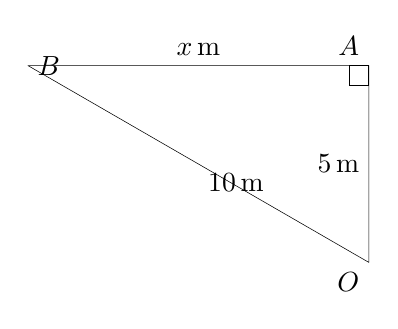
\begin{tikzpicture}
		\tkzDefPoints{0/0/O,0/2.5/A}
		\tkzDefShiftPoint[A](1,0){b}

		\tkzInterLC[R](A,b)(O,5cm)
		\tkzGetSecondPoint{B}

		\tkzDrawPolygon(O,A,B)
		\tkzLabelPoints[below left](O)
		\tkzLabelPoints[above left](A)
		\tkzLabelPoints[right](B)
		\tkzLabelLine[left](O,A){$\SI{5}{m}$}
		\tkzLabelLine[below right](O,B){$\SI{10}{m}$}
		\tkzLabelLine[above](A,B){$\SI[parse-numbers=false]{x}{m}$}
		\tkzMarkRightAngle(O,A,B)
	\end{tikzpicture}
\end{wrapfigure}
If we plot the position of Farmer Pearson's house ($O$), Bessie's starting position ($A$), and Bessie's position when she is exactly $10$ meters away from the house ($B$), we can see that the points form a right triangle.
We can use the Pythagorean theorem to find $x$, which is how far Bessie moved in meters.
$x^2 + 5^2 = 10^2$, so $x^2 = 100 - 25 = 75$ and $x = \sqrt{75}$.
Time is distance divided by speed and Bessie moved at $2$ meters per second, so it took her $\frac{\sqrt{75}}{2}$ seconds to get $10$ meters away from the house.
The square root can be simplified since $75$ is a multiple of a perfect square, so the final answer is
\[
	\frac{\sqrt{75}}{2} = \frac{\sqrt{25 \cdot 3}}{2} = \frac{\sqrt{25}\sqrt{3}}{2} = \boxed{\frac{5\sqrt{3}}{2}}
\]
Alternatively, we can also use the special right triangle ratios instead of the Pythagorean theorem.
This right triangle is a $30$-$60$-$90$ triangle because $OA$ is half of $OB$.
In a $30$-$60$-$90$ triangle, the length of the longer leg is $\sqrt{3}$ times the length of the shorter leg, so $x = 5\sqrt{3}$ and we also get $\frac{5\sqrt{3}}{2}$ seconds as the answer.

\section{Moss-cow}
Let $a$ be the number of hours Bessie spent on the plane and $b$ be the number of hours Bessie spent on the train.
$a + b = 19.5$, and $560a + 60b = 1600$, since $560a$ is the distance she travelled by plane and $60b$ is the distance she travelled by train.
We can multiply the first equation by $60$ to get $60a + 60b = 1170$, then subtract this from the second equation to get $560a + 60b - 60a - 60b = 1600 - 1170$, so $500a = 430$.
Therefore, $a = \frac{430}{500} = \frac{43}{50}$.
$\frac{43}{50}$ hours is $\frac{43}{50} \cdot 60 = 51.6$ minutes, which rounds to $52$ minutes.

\section{Look Mom No Proof!}
The first rule in the paper checks for divisibility by $2$, the second rule checks for divisibility by $5$, and the third rule checks for divisibility by $3$.
Therefore, the paper is claiming that any integer greater than $5$ which is not a multiple of $2$, $3$, or $5$ is either a prime or a power of a prime.
To disprove this, we can find a number that is not a multiple of $2$, $3$, or $5$ and is not a prime or a power of a prime.
Our number must have at least two different prime factors in order for it to not be a power of a prime, and we can't have $2$, $3$, or $5$ as prime factors.
We can take any two primes that aren't $2$, $3$, or $5$ and multiply them together.
The smallest two primes that aren't $2$, $3$, or $5$ are $7$ and $11$, so the smallest counterexample is $7 \cdot 11 = 77$.

\section{Completely Organic Watermelons (C.O.W)}
The simplest way to solve this problem is to use complementary counting.
First, there are $\binom{18}{3} = \frac{18 \cdot 17 \cdot 16}{3 \cdot 2} = 816$ ways to choose any $3$ watermelons out of $18$ watermelons.
Now we'll count the number of ways to choose three watermelons of the same size.
There are $\binom{5}{3}$ ways to choose three large watermelons, $\binom{6}{3}$ ways to choose three medium watermelons, and $\binom{7}{3}$ ways to choose three small watermelons, for a total of $\binom{5}{3} + \binom{6}{3} + \binom{7}{3} = 65$.
The number of ways to choose three watermelons that aren't all the same size is therefore $816 - 65 = 751$.

\section{Cowtapult}
\begin{wrapfigure}{R}{0.4\linewidth}
	\vspace{-30pt}
	\centering
	\includegraphics[scale=0.1]{cowtapult_solution.png}
	\vspace{-30pt}
\end{wrapfigure}
First, extend the paths of the hay bale and the enemy cart until they intersect at the point where the hay bale hits the cart.
Also extend the dotted line pointing north from the position of the hay bale launcher until it intersects the path of the cart.
The path of the hay bale, the path of the cart, and the dotted line form a $30$-$60$-$90$ right triangle.
The length of the long leg (the dotted line) is $80 - 15 = 65$ meters.
We can use the special right triangle ratios to find the length of the short leg.
The ratio between the short leg and the long leg in a $30$-$60$-$90$ triangle is $\frac{1}{\sqrt{3}}$, so the length of the short leg is $\frac{65}{\sqrt{3}}$ meters.
This means that the cart traveled a total of $50 + \frac{65}{\sqrt{3}}$ meters.
The time it took for the cart to travel this far is $\frac{50 + \frac{65}{\sqrt{3}}}{10} = 5 + \frac{13}{2\sqrt{3}}$ seconds.
The distance which the hay bale traveled is $65 \cdot \frac{2}{\sqrt{3}}$, since the ratio between the hypotenuse and the long leg in a $30$-$60$-$90$ triangle is $\frac{2}{\sqrt{3}}$.
It took $\frac{65 \cdot \frac{2}{\sqrt{3}}}{20} = \frac{13}{2\sqrt{3}}$ seconds for the hay bale to hit the cart after it's launched.
Therefore, the hay bale must be launched after $5 + \frac{13}{2\sqrt{3}} - \frac{13}{2\sqrt{3}} = 5$ seconds.

\section{woC}
The expected value is the sum of the value of each outcome multiplied by its probability.
In this problem, the probability of every outcome is equal, so this is the same as the average of all the outcomes.
The number of outcomes is $8375 - 1000 + 1 = 8376$, so we just need to find the sum of all the outcomes.
To do this, we can find the sum of each digit of the outcomes separately, multiply them by powers of ten, and add them together.

The sum of the units digit of the reversed numbers is the sum of the thousands digit of the numbers from $1000$ to $8375$.
For each of the digits from $1$ to $7$, there are $100$ numbers with that digit in the thousands place.
There are $376$ numbers with $8$ as the thousands digit, so the total sum is $(1 + 2 + 3 + 4 + 5 + 6 + 7) \cdot 1000 + 8 \cdot 376 = 31008$.

Similarly, the sum of the tens digit of the reversed numbers is the sum of the hundreds digit of the original numbers.
If the thousands digit is from $1$ to $7$, then the hundreds digit can be anything.
For each of the $10$ possible hundreds digits, there are $7$ possible values for the thousands digit and $100$ possible values for the tens and units digits.
If the thousands digit is $8$, then the hundreds digit can be $0$, $1$, $2$, or $3$.
If it is less than $3$, than the last two digits have $100$ possible values.
If the hundreds digit is $3$, then the last two digits have $76$ possible values.
Therefore, the sum of the hundreds digits is $(0 + 1 + 2 + 3 + 4 + 5 + 6 + 7 + 8 + 9) \cdot 7 \cdot 100 + (0 + 1 + 2) \cdot 100 + 3 \cdot 76 = 32028$.

For the sum of the tens digit, if the first two digits are less than $83$, then the tens digit can have any value and there are $10$ possible values for the units digit.
If the first two digits is $83$ and the tens digit is less than $7$, then the units digit has $10$ possible values, and if the tens digit is $7$, then the units digit has $6$ possible values.
So the sum of the tens digit is $(0 + 1 + 2 + 3 + 4 + 5 + 6 + 7 + 8 + 9) \cdot 73 \cdot 10 + (0 + 1 + 2 + 3 + 4 + 5 + 6) \cdot 10 + 7 \cdot 6 = 33102$.

Lastly, if the first three digits are less than $837$, then the units digit can have any value, and if the first three digit is $837$, then the units digit can be from $0$ to $5$, so the sum is $(0 + 1 + 2 + 3 + 4 + 5 + 6 + 7 + 8 + 9) \cdot 737 + 0 + 1 + 2 + 3 + 4 + 5 = 33180$.

The sum of the reversed numbers is $33180 \cdot 1000 + 33102 \cdot 100 + 32028 \cdot 10 + 31008 = 36841488$, which means the expected value is $\frac{36841488}{8375 - 1000 + 1} = \frac{2302593}{461}$.

\section{Baa Baa Bazaar}
\begin{wrapfigure}{r}{0.5\linewidth}
	\vspace{-20pt}
	\centering
	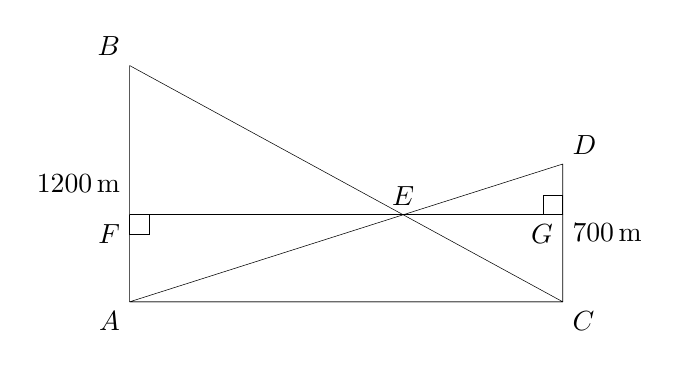
\begin{tikzpicture}[scale=0.25]
		\tkzDefPoint(0,0){A}
		\tkzDefPoint(0,12){B}
		\tkzDefPoint(22,0){C}
		\tkzDefPoint(22,7){D}
		\tkzDrawPolygon(A,B,C)
		\tkzDrawPolygon(A,C,D)
		\tkzLabelSegment[left](A,B){\SI{1200}{m}}
		\tkzLabelSegment[right](C,D){\SI{700}{m}}
		\tkzLabelPoints[below left](A)
		\tkzLabelPoints[above left](B)
		\tkzLabelPoints[below right](C)
		\tkzLabelPoints[above right](D)
		\tkzInterLL(A,D)(B,C)
		\tkzGetPoint{E}
		\tkzLabelPoints[above](E)
		\tkzDefLine[orthogonal=through E](A,B)
		\tkzInterLL(A,B)(E,tkzPointResult)
		\tkzGetPoint{F}
		\tkzInterLL(F,E)(C,D)
		\tkzGetPoint{G}
		\tkzDrawSegment(F,G)
		\tkzLabelPoints[below left](F,G)
		\tkzMarkRightAngle[size=1](E,F,A)
		\tkzMarkRightAngle[size=1](E,G,D)
	\end{tikzpicture}
	\vspace{-20pt}
\end{wrapfigure}
First, we'll label the points in the diagram as shown.
We drew a horizontal line passing through $E$, and labeled its intersection points with $\overline{AB}$ and $\overline{CD}$.
First, $\angle BEA$ and $\angle CED$ are congruent, since they are vertical angles.
$\angle BAE$ and $\angle CDE$ are congruent because they are alternate interior angles and the $\overline{AB} \parallel \overline{CD}$.
Therefore, $\triangle ABE$ and $\triangle DCE$ are similar by AA similarity.
$\overline{AB}$ and $\overline{DC}$ correspond to each other and the ratio of their lengths is $\frac{\SI{700}{m}}{\SI{1200}{m}} = \frac{7}{12}$, so this is the ratio between all pairs of corresponding segments in these triangles.
The length that we need to find is the same as the length of $\overline{AF}$.
This corresponds to $\overline{DG}$, so the ratio between the length of $\overline{DG}$ and the length of $\overline{AF}$ is $\frac{7}{12}$.
$FA = GC$ so the ratio between $DG$ and $GC$ is $\frac{7}{12}$ and their sum is $\SI{700}{m}$, so $\frac{DG}{GC} = \frac{7}{12}$ and $DG + GC = \SI{700}{m}$.
We can solve this system of equations using substitution.
The first equation is equivalent to $DG = \frac{7}{12}GC$.
Substituting this into the second equation gives $\frac{7}{12}GC + GC = \SI{700}{m}$, so $\frac{19}{12}GC = \SI{700}{m}$ and $GC = \frac{12}{19} \cdot \SI{700}{m} = \SI[parse-numbers=false]{\frac{8400}{19}}{m}$.
This is the height of the intersection point.

\section{The Great Cow Chase}
\begin{wrapfigure}{r}{0.25\linewidth}
	\centering
	\vspace{-20pt}
	\begin{tikzpicture}
		\tkzDefPoint(0,0){A}
		\tkzDefPoint(0,3){B}

		\tkzDefTriangle[school](B,A)
		\tkzGetPoint{C}

		\tkzDrawPolygon(A,B,C)
		\tkzLabelPoints[below left](A)
		\tkzLabelPoints[above](B)
		\tkzLabelPoints[right](C)
		\tkzMarkRightAngle(B,A,C)
	\end{tikzpicture}
\end{wrapfigure}
Rancher Cedric needs to move from his starting point to some point on Kiran's path, and he needs to reach the point on Kiran's path before Kiran passes it.
Rancher Cedric should always move in a straight line, because if he doesn't move in a straight line he would be able to reach the point on Kiran's path faster by moving in a straight line.
Also, it wouldn't make sense for Rancher Cedric to reach a point on Kiran's path before Kiran gets there, because then Rancher Cedric could have moved to an earlier point on Kiran's path.
Let's plot Kiran's starting position ($A$), Rancher Cedric's starting position ($B$) and the point where Rancher Cedric catches Kiran ($C$).
These points form a right triangle.
Rancher Cedric is twice as fast as Kiran, so his path is twice as long as Kiran's path.
This means that $\triangle BAC$ is a $30$-$60$-$90$ right triangle because its hypotenuse is twice as long as one of its legs.
We know the ratios between the side lengths of a $30$-$60$-$90$ right triangle and we know $AB$, so we can find $AC$, which is the distance that Kiran travelled.
The ratio between the length of the short leg and the length of the long leg in a $30$-$60$-$90$ right triangle is $\frac{1}{\sqrt{3}}$, so Kiran travelled $\frac{10}{\sqrt{3}}$ miles.
Kiran moves at $15$ miles per hour, so it took $\frac{10}{15\sqrt{3}} = \frac{2}{3\sqrt{3}}$ hours for Rancher Cedric to catch Kiran.
We multiply by $3600$ to convert to minutes, so the answer is $\frac{2 \cdot 3600}{3\sqrt{3}} \approx 1386$ seconds.

\section{Rowdy Cow}
The area of an equilateral triangle with side length $s$ is $s^2 \frac{\sqrt{3}}{4}$, so the area of the pen is $500^2 \cdot \frac{\sqrt{3}}{4} = 62500\sqrt{3}$ square meters.
Half of this is $31250\sqrt{3}$.
The area which Kiran can reach will be in the shape of a sector with an angle of $\ang{60}$.
This sector is one-sixth of a circle with the same radius, so if $r$ is the length of the rope in meters, the area is $\frac{\pi r^2}{6}$.
We have $\frac{\pi r^2}{6} = 31250\sqrt{3}$, so $r = \sqrt{\frac{31250\sqrt{3} \cdot 6}{\pi}} \approx 321.52$.
Therefore, the rope is $321.52$ meters long.

\section{My Cow Ate My Homework}
We can treat the two values $a$ and $b$ as the coordinates for a point on a plane.
Randomly choosing the values for $a$ and $b$ is the same as randomly choosing a point in a $18$ by $18$ square centered on the origin.
We can expand the left side of the inequality to get $a^2 + 2ab + b^2 \leq 2ab + 9$, and subtracting $2ab$ from both sides gives $a^2 + b^2 \leq 9$.
A pair of values satisfy this inequality if and only if the point $(a, b)$ is at most $3$ units away from the origin, so this inequality represents the set of all points inside a circle with radius $3$ centered on the origin.
The circle is completely within the $18$ by $18$ square, so the probability that a random point is in the circle is the area of the circle divided by the area of the square.
The area of the circle is $\pi \cdot 3^2 = 9\pi$ and the area of the square is $18^2$, so the probability is $\frac{9\pi}{18^2} = \frac{\pi}{36}$.

\section{Cowloring}
We will split this problem into three cases.

First, we'll count the number of coloring schemes that are $\ang{90}$ rotationally symmetric.
In this case, the color of each region except the center one must be the same as the color of the three other corresponding regions.
For example, the color of the topmost region, the leftmost region, the rightmost region, and the bottommost region must be the same.
We really only have $4$ regions here, so the number of coloring schemes is $3^4$.

Next, we'll count the coloring schemes that are $\ang{180}$ rotationally symmetric but not $\ang{90}$ rotationally symmetric.
In order for the coloring scheme to be $\ang{180}$ symmetric, opposing regions must have the same color.
We have six pairs of regions which must have the same color plus the center, so the number of coloring schemes is $3^7$.
This includes coloring schemes which are also $\ang{90}$ symmetric, so we subtract these to get $3^7 - 3^4$.
Every coloring scheme that is $\ang{180}$ symmetric has $2$ different orientations, so this counts each of them twice.
Therefore, we will divide by $2$ to get $\frac{3^7 - 3^4}{2}$.

Finally, we'll count the coloring schemes which are not rotationally symmetric in a similar way.
There are $13$ regions, so there are $3^{13}$ ways to choose colors for the regions.
$3^7$ of these are rotationally symmetric, so we subtract them.
Then we divide by $4$ because each coloring scheme has $4$ different orientations to get $\frac{3^{13} - 3^7}{4}$.
The total is $3^4 + \frac{3^7 - 3^4}{2} + \frac{3^{13} - 3^7}{4} = 399168$.
\end{document}
